\documentclass[11pt]{article}

\usepackage{amsmath}
\usepackage{amssymb} 
\usepackage{textcomp}
\usepackage{float}
\usepackage[top=0.8in, bottom=0.8in, left=0.8in, right=0.8in]{geometry}
\usepackage{graphicx}
\usepackage{wrapfig}
\graphicspath{ {./} }
% Add other packages here %


% Put your group number and names in the author field %
\title{\bf Excercise 3\\ Implementing a deliberative Agent}
\author{Group \textnumero : 90  Kyle Gerard, Yann Bolliger}


% N.B.: The report should not be longer than 3 pages %


\begin{document}
\maketitle

\section{Model Description}

\subsection{Intermediate States}
Mathematically seen our state contains all positions of all the objects on the 
map. That means the current position of the agent, all the tasks the agent has already picked up
and all the tasks to be picked up yet. This could be written as the following state space:

$$
\mathcal{S} = \mathcal{C} 
\times
\{ A_{carried} : A_{carried} \subseteq \mathcal{T} \}
\times
\{ A_{pending} : A_{pending} \subseteq \mathcal{T} , 
  A_{pending}  \cap A_{carried}  = \emptyset
  \}
$$

where $\mathcal{C} $ is the set of cities and $ \mathcal{T}$ is the overall set 
of tasks. 

\subsection{Goal State}
A goal state is reached when all packets/tasks are delivered. Therefore it is 
defined as:

$$
\mathcal{S}_{goal} =  \{  (C, A_{carried}, A_{pending}) \in  \mathcal{S} : 
A_{carried} = \emptyset \wedge A_{pending} = \emptyset \} \subset  \mathcal{S}
$$

\subsection{Actions}
At each state there are up to three possible actions: move, pickup, deliver. 
They all have some conditions on the current state:

\begin{itemize}
  \item
  The agent can move only to neighbors of the current city encoded in the state. 
  This changes the city for the next state, the rest stays the same.
  
    \item
  The agent can deliver a task if $ \exists T \in A_{carried}$ which has 
  to be delivered at the current city of the agent.
  Then this task is removed from $A_{carried}$ for the next state.
  
  \item
  The agent can pickup a task only if $\exists T \in A_{pending} $ which has to 
  be picked up from the current city of the agent and if 
  $\sum_{T \in A_{carried} } \text{weight} (T) < $ maximal capacity of the 
  vehicle.
  In that case $T$ is removed from  $A_{pending}$  and added to $A_{carried}$ 
  for the next state.
\end{itemize}



\section{Implementation}

\subsection{BFS}
We closely followed the BFS algorithm. However, instead of stopping the 
search at the first goal node, we traverse the entire tree and take the plan 
with the minimal cost at the end. 

In order to make this memory consuming search fast, there are some 
important keypoints. We defined a specialised node class that acts as nodes in 
the search tree. These nodes don't only store the formal \texttt{State} of the 
agent but also the plan up to this state and the corresponding cost. This 
saves us from recomputing the entire two properties for each search node.

Another small point is cylce detection. This is where we prevent reconsidering 
states we have already seen unless we find them with a smaller cost.

The most important speedup comes however from choosing the correct data-structures.
For $\mathcal{O}(1)$ lookups of states for cycle detection and other lookups we 
always use a \texttt{HashMap} together with the hash function of the class 
\texttt{State}.
For the search agenda queue we rather use linked list in order to prevent costly 
array copying. This makes our BFS reasonably fast for up to 11 tasks.

\subsection{A*}
As in BFS, we closely followed to algorithm given and made use of an admissible 
heuristic. This lets us do simple cycle detection because we know that we find a 
state optimally in the first place. Again, we wrote a specialised \texttt{Node} 
class that keeps track of the state, the plan, the cost and the heuristic in the 
search tree.

We also reused \texttt{HashMap} for cycle detection but here,
 we leveraged even more of Java's rich collection API. In fact, the search 
agenda queue is a \texttt{PriorityQueue}. This is a binary heap implementation 
and works with the \texttt{compareTo} metod of \texttt{Node}. Therefore it automatically 
gives us the search node with the lowest $f()$ value in $\mathcal{O}(\log n)$ 
time. Which is an immense advantage compared to the approach where the entire 
list of search nodes is sorted in $\mathcal{O}(n \log n)$ time!

\subsection{Heuristic Function}
The heuristic in our A*-Algorithm must be admissible. It is defined as:
$$
h(S = (C, A_{carried}, A_{pending})) = \max (h(A_{carried}), h(A_{pending})) 
$$$$
h(A_{carried}) = \max_{T \in A_{carried}} \text{distance}(C, \text{destination}(T))
$$$$
h(A_{pending}) = \max_{T \in A_{pending}} \text{distance}(C, \text{origin}(T)) + 
\text{distance}(\text{origin}(T), \text{destination}(T))
$$

This is admissible because if the agent has at least one pending task, it has \textit{at least}
to go to the task's origin, pick it up and deliver it. In that case the heuristic exactly 
calculates the cost. If the agent has more tasks, the heuristic will underestimate the cost. 
The same is true if the agent only has one carried task. Therefore the heuristic 
is admissible.

--> monotonic, optimal?


\section{Results}

\subsection{Experiment 1: BFS and A* Comparison}
% Compare the two algorithms in terms of: optimality, efficiency, limitations %
% Report the number of tasks for which you can build a plan in less than one minute %

\subsubsection{Setting}
% Describe the settings of your experiment: topology, task configuration, etc. %
The config file used was the one given in the handout called deliberative.xml with rngSeed left as is at 23456. Both the BFS and ASTAR algorithms were used. For each algorithm, we measured the time to compute the optimal plan as a function of the number of tasks to pickup nd deliver.  

\subsubsection{Observations}
% Describe the experimental results and the conclusions you inferred from these results %
\begin{center}
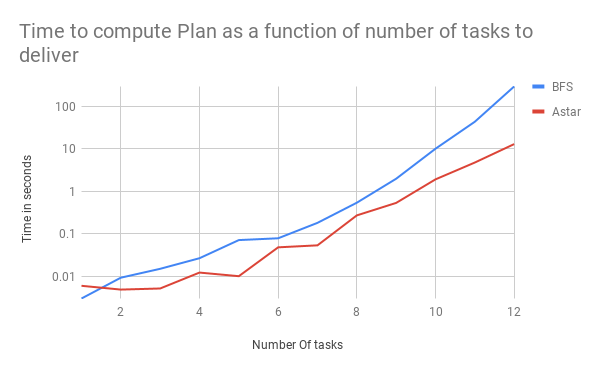
\includegraphics[width=12cm]{time.png}
\end{center}
As seen in the graph above, both the ASTAR and BFS algorithms' time to compute the optimal plan grow exponentially as a function of the number of tasks to deliver. We also remark that the ASTAR algorithm runs significantly faster than BFS. Using BFS we can build a plan with 11 tasks in 38 seconds. Using ASTAR we can build a plan with 13 tasks in 15 seconds. Therefore, even though both algorithms compute the optimal plan, ASTAR is more efficient than BFS. However as both algorithm's complexity is exponential, both algorithms are of limited use (much too slow) as the number of tasks increases.

\subsection{Experiment 2: Multi-agent Experiments}
% Observations in multi-agent experiments %

\subsubsection{Setting}
% Describe the settings of your experiment: topology, task configuration, etc. %
Here we use the ASTAR algorithm for all agents because it is faster than BFS at calculating the optimal plan. Still using the deliberative.xml config file, we examine the behavior of agents depending on the number of agents in the environment.
\subsubsection{Observations}
% Describe the experimental results and the conclusions you inferred from these results %
\begin{center}
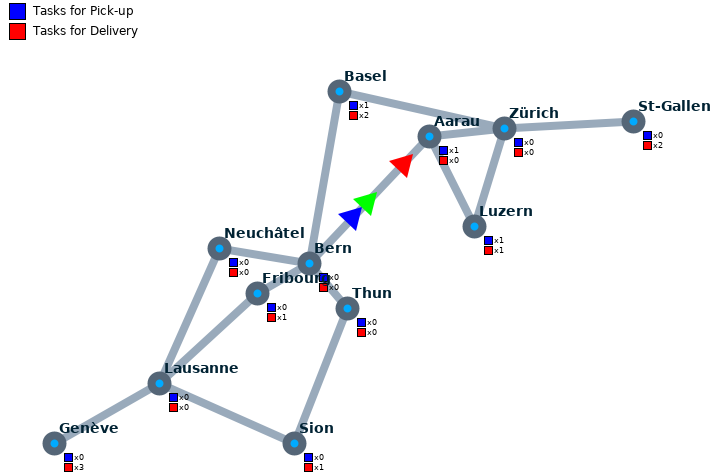
\includegraphics[width=6cm]{follow.png}
\end{center}
With more than one agent in the environment we rapidly observe that agents no longer act optimally. Indeed, their "optimal" plans computed by the ASTAR algorithm does not take into the other agents' plans. This means that agents will travel to  city to pickup a task even though another agent is closer to the city and thus will pickup the task first. In the figure above we see 3 agents going to the same pickup city even though there is only one task to be picked up. In this case the optimal plan would be to not try and pickup a task from a city when will reach it earlier. 
\end{document}
